%\documentclass[cjk,slidestop,compress,brown]{beamer}
\documentclass[cjk,t,compress]{beamer}
%\documentclass[cjk,slidestop,compress]{beamer}

\usepackage{amsmath}
\usepackage{amssymb}
\usepackage{amsthm}

\mode<presentation>
{
%	\usetheme{Hannover}
%	\usetheme{Goettingen}
%   \usetheme{Boadilla}
%	\usetheme{Szeged}
%	\usetheme{Singapore}
%	\usetheme{CambridgeUS}
	\setbeamercovered{dynamic}
	\usefonttheme[hoptionsi]{serif}
%  \usecolortheme[green]{structure}
}

\usepackage{amsmath}
\usepackage{amssymb}
\usepackage{amsthm}
\usepackage{mathtools}

\mode<presentation>
{
%	\usetheme{Hannover}
%	\usetheme{Goettingen}
%   \usetheme{Boadilla}
%	\usetheme{Szeged}
%	\usetheme{Singapore}
%	\usetheme{CambridgeUS}
	\setbeamercovered{dynamic}
	\usefonttheme[hoptionsi]{serif}
%  \usecolortheme[green]{structure}
}

\usepackage[latin1]{inputenc}
\usepackage[spanish]{babel}
%\usepackage{xcolor}
%\usepackage[dvips]{color}
%\usepackage{multicol}
%\usepackage{subfigure}

\definecolor{MyDarkBlue}{rgb}{0 0.08 0.45}
\definecolor{MyDarkOrange}{rgb}{1 0.5 0}
\definecolor{MyDarkGreen}{rgb}{0 0.25 0}
\definecolor{MyDarkTerracota}{rgb}{0.5 0 0}
\definecolor{MyDarkGrey}{rgb}{0.25 0.25 0.25}

% ---------------------------------------------
%				Fields
% ---------------------------------------------
\newcommand{\Indicator}{\operatorname{\mathds{1}}}
\newcommand{\Indic}{\operatorname{\field{I}}}
\newcommand{\field}[1]{\mathbb{#1}} 
\newcommand{\C}{\field{C}}
\newcommand{\E}{\field{E}} 
\newcommand{\R}{\field{R}}
\newcommand{\inccoin}{\Delta c}
\newcommand{\incy}{\Delta y}

% ---------------------------------------------
%				Observables
% ---------------------------------------------
\newcommand{\barx}{\bar{x}}
\newcommand{\barX}{\bar{X}}
\newcommand{\boldc}{\boldsymbol{c}}
\newcommand{\boldC}{\boldsymbol{C}}
\newcommand{\boldm}{\boldsymbol{m}}
\newcommand{\boldM}{\boldsymbol{M}}
\newcommand{\boldr}{\boldsymbol{r}}
\newcommand{\boldR}{\boldsymbol{R}}
\newcommand{\boldx}{\boldsymbol{x}}
\newcommand{\boldX}{\boldsymbol{X}}
\newcommand{\boldy}{\boldsymbol{y}} 
\newcommand{\boldY}{\boldsymbol{Y}}
\newcommand{\boldu}{\boldsymbol{u}} 
\newcommand{\boldU}{\boldsymbol{U}}
\newcommand{\boldzero}{\boldsymbol{0}} 
\newcommand{\boldA}{\boldsymbol{A}} 
\newcommand{\boldW}{\boldsymbol{W}}

% ---------------------------------------------
%				Parameters
% ---------------------------------------------
\newcommand{\Piexp}{\Pi^{e}} 
\newcommand{\Pidelta}{\delta^{\Pi}} 

\newcommand{\rhoexp}{\rho^{e}} 
\newcommand{\rhodelta}{\delta^{\rho}} 

\newcommand{\tauexp}{\tau^{e}} 
\newcommand{\taudelta}{\delta^{\tau}} 

\newcommand{\thetaexp}{\theta^{e}} 
\newcommand{\thetadelta}{\delta^{\theta}} 

\newcommand{\tk}{t:(t+k)} 

\newcommand{\boldlambda}{\boldsymbol{\lambda}} 
\newcommand{\boldLambda}{\boldsymbol{\Lambda}} 
\newcommand{\boldmu}{\boldsymbol{\mu}} 
\newcommand{\boldMu}{\boldsymbol{\Mu}} 
\newcommand{\boldsigma}{\boldsymbol{\sigma}} 
\newcommand{\boldSigma}{\boldsymbol{\Sigma}} 
\newcommand{\boldphi}{\boldsymbol{\phi}} 
\newcommand{\boldPhi}{\boldsymbol{\Phi}} 
\newcommand{\boldbeta}{\boldsymbol{\beta}}
\newcommand{\boldBeta}{\boldsymbol{\Beta}}
\newcommand{\boldtheta}{\boldsymbol{\theta}}
\newcommand{\boldTheta}{\boldsymbol{\Theta}}
\newcommand{\bolds}{\boldsymbol{s}} 
\newcommand{\boldS}{\boldsymbol{S}} 

%   --------------------------------
%               Notation
%   --------------------------------
\newcommand{\lik}{\mathrm{lik}}
\newcommand{\diagop}{\text{diag}} 
\newcommand{\logistic}{\operatorname{\text{logistic}}}
\newcommand{\logit}{\operatorname{\text{logit}}}
\newcommand{\dom}{\operatorname{\text{dom}}}
\newcommand{\ran}{\operatorname{\text{ran}}}
\renewcommand{\inf}{\operatorname{\text{inf}}}
\newcommand{\ind}{\operatorname{\text{ind}}}
\newcommand{\iid}{\operatorname{\text{iid}}}
\newcommand{\cind}{\operatorname{\text{c.i.}}}
\newcommand{\wport}{\text{w}}

\renewcommand{\Pr}{\field{P}}
\newcommand{\dd}{\mathrm{d}}
\newcommand{\Borel}{\operatorname{\mathscr{B}}}
\newcommand{\Filtration}{\operatorname{\mathscr{F}}}
\newcommand{\expec}{\operatorname{\field{E}}}
%\newcommand{\media}{\operatorname{\text{media}}}
%\newcommand{\moda}{\operatorname{\text{moda}}}
%\renewcommand{\var}{\operatorname{\text{var}}}
%\newcommand{\prec}{\operatorname{\text{prec}}}
%\newcommand{\cov}{\operatorname{\text{cov}}}
%\newcommand{\corr}{\operatorname{\text{corr}}}
%\newcommand{\varmodel}{\operatorname{\text{VAR}}}

\renewcommand{\sin}{\operatorname{\text{sin}}}
\renewcommand{\cos}{\operatorname{\text{cos}}}
\renewcommand{\tan}{\operatorname{\text{tan}}}
\renewcommand{\arctan}{\operatorname{\text{arctan}}}
\renewcommand{\exp}{\operatorname{\text{exp}}}
\renewcommand{\log}{\operatorname{\text{log}}}
\renewcommand{\arg}{\operatorname{\text{arg}}}
\renewcommand{\min}{\operatorname{\text{min}}}
\renewcommand{\max}{\operatorname{\text{max}}}
\renewcommand{\lim}{\operatorname{\text{lim}}}
\newcommand{\limite}{\operatornamewithlimits{lim}}
\renewcommand{\det}{\operatorname{\text{det}}}
\renewcommand{\dim}{\operatorname{\text{dim}}}
\newcommand{\sign}{\operatorname{\text{sign}}}
\newcommand{\argmax}{\operatornamewithlimits{arg\,max}}
\newcommand{\argmin}{\operatornamewithlimits{arg\,min}}
\newcommand{\diagbloq}{\operatorname{\text{diagbloq}}}
\newcommand{\rr}{\operatorname{\textsc{R}}}

\newcommand{\ie}{{\it i.e. }} 
\newcommand{\aka}{{\it a.k.a. }} 
\newcommand{\eg}{{\it e.g. }} 
\newcommand{\ala}{{\it \`{a}~la }} 
\newcommand{\visavis}{{\it vis-\`{a}-vis }}

\newcommand{\inpc}{\text{INPC}}
\newcommand{\igae}{\text{IGAE}}
\newcommand{\Pib}{\text{PIB}}
\newcommand{\tiie}{\text{TIIE}}
\newcommand{\export}{\text{Exportaciones}}
\newcommand{\import}{\text{Importaciones}}
\newcommand{\usip}{\text{IP}^{\usa}}
\newcommand{\remMX}{\text{Rem}^{\usa}}
\newcommand{\itaen}{\text{ITAE}}
\newcommand{\itaee}{\text{ITAEE}}
\newcommand{\usa}{\text{EEUU}}
\newcommand{\dsge}{\operatornamewithlimits{DSGE}}

% ---------------------------------------------
%				Distributions
% ---------------------------------------------

\newcommand{\WiD}{\operatorname{\text{Wi}}}
\newcommand{\WiInvD}{\operatorname{\text{Wi-Inv}}}
\newcommand{\WeD}{\operatorname{\text{We}}}
\newcommand{\WeNormD}{\operatorname{\text{We-N}}}
\newcommand{\ExpD}{\operatorname{\text{Exp}}}
\newcommand{\GeoD}{\operatorname{\text{Geo}}}
\newcommand{\StD}{\operatorname{\text{St}}}
\newcommand{\NormD}{\operatorname{\text{N}}}
\newcommand{\GaD}{\operatorname{\text{Ga}}}
\newcommand{\BerD}{\operatorname{\text{Ber}}}
\newcommand{\BinD}{\operatorname{\text{Bin}}}
\newcommand{\BeD}{\operatorname{\text{Be}}}
\newcommand{\UniD}{\operatorname{\text{U}}}
\newcommand{\DirD}{\operatorname{\text{Dir}}}
\newcommand{\IG}{\operatorname{\text{InG}}}
\newcommand{\IncGa}{\operatorname{\text{IGa}}}
\newcommand{\IGa}{\operatorname{\text{InGa}}}
\newcommand{\PoD}{\operatorname{\text{Po}}}
\newcommand{\BS}{\operatorname{\text{BS}}}
\newcommand{\DP}{\operatorname{\text{DP}}}
\newcommand{\PaD}{\operatorname{\text{Pa}}}


%   --------------------------------
%               Directories
%   --------------------------------
\graphicspath{{../figures/}}
\DeclareGraphicsExtensions{.pdf,.jpeg,.png,.jpg}

\title[C\'alculo Actuarial III]
{	ACT-11302: C\'alculo Actuarial III\\
	{\large Sesi\'on 09a: Teor\'ia de ruina}
}

\author[Mart\'inez-Ovando]{
{	\footnotesize
	\textcolor{MyDarkGreen}{Juan~Carlos Mart\'inez-Ovando}}
}

\institute[ITAM]
{	\textcolor{MyDarkGrey}{
	ITAM}
}

\date[ ] % (optional)
{	\scriptsize
	\textcolor{MyDarkGrey}{Oto\~no 2019}
}

%	--------------------------------------------
%									Titlepage
%	--------------------------------------------
\begin{document}
\sffamily
%	-------------		FRAME		--------------------
\begin{frame}[fragile]
	\frametitle{}
	\titlepage
\end{frame}


%
%	Section: Monto agregado de siniestros
%
\section{1. Teor\'ia de ruina}
%	-------------		FRAME		--------------------
\begin{frame}[fragile]
	\frametitle{}
	\vspace{5.5cm}
	\begin{flushright}
		\textcolor{MyDarkBlue}{\Large \bf 1. Teor\'ia de ruina}
	\end{flushright}
\end{frame}

%
%	Sub-section: Antecedentes
%
\subsection{1.1. Teor\'ia de ruina: Preliminares}
%	-------------		FRAME		--------------------
\begin{frame}[fragile]
	\frametitle{1.1. Teor\'ia de ruina: Preliminares}
	\scriptsize  	
		
		\vspace{0.1cm}
		\begin{block}<+->{Antecedentes}
		\vspace{0.1cm}
		\begin{itemize}
		  \item Una aseguradora se vuelve \textcolor{blue}{insolvente} (o est\'a en \textcolor{blue}{quiebra}) cuando sus egresos son mayores que sus ingresos
		  
		  \item Bajo ciertas condiciones sobre el \textcolor{blue}{capital inicial} y los \textcolor{blue}{flujos de efectivo operativos}, el {\bf tiempo} y el {\bf tama\~no} de la pr\'oxima quiebra son naturalmente dos variables aleatorias
		  
		  \item La \textcolor{blue}{\bf teor\'ia de ruina} tiene como objetivo estudiar las conexiones entre estas condiciones iniciales y las distribuciones de estas variables, para cuantificar la posibilidad de ruina y controlarla.
		\end{itemize}
		\end{block}

\end{frame}

%	-------------		FRAME		--------------------
\begin{frame}[fragile]
	\frametitle{1.1. Teor\'ia de ruina: Preliminares}
	\scriptsize  	
		
		\vspace{0.1cm}
		\begin{block}<+->{Preliminares}
		\vspace{0.1cm}
		La {\bf teoria de ruina} consiste en el estudio de procesos temporales en $t$ del {\bf capital} de una empresa, denotado por $U(t)$, en particular para una {\bf empresa aseguradora}.

		El {\bf capital}, en si mismo, es definico a traves de una relacion contable, donde en un $t$ particular se cumple
$$
U(t) = U(0) + \Pi(t) - S(t),
$$
siendo 
		\begin{itemize}
		  \item $U(0)$ el {\bf capital inicial} de operacion en el tiempo $t=0$,

		  \item $\Pi(t)$ el {\bf monto acumulado por derechos} (a.k.a. por suscripcion) entre $t=0$ y $t$

		  \item $S(t)$ el {\bf monto acumulado de obligaciones} (a.k.a. reclamos) entre $t=0$ y $t$
		\end{itemize}

	\vfill
	\emph{$\bullet$ El estudio de $\Pi(t)$ compete al `estudio de riesgos de mercado`, mientras que $S(t)$ compete al `estudio de riesgo operacional` (nuestro curso).}

	\vfill
	\emph{$\bullet$ Nosotros supondremos que $U(0)$ y $\Pi(t)$, para todo $t\geq 0$ son dados.}

	\vfill
	\emph{$\bullet$ Suponiendo que $U(0)$ y $\Pi(t)$ son dados, y $S(t)$ desconocido/aleatorio, tendremos que $U(t)$ es en si mismo aleatorio.}
		\end{block}

\end{frame}

%	-------------		FRAME		--------------------
\begin{frame}[fragile]
	\frametitle{1.1. Teor\'ia de ruina: Preliminares}
	\scriptsize  	

		\vspace{0.1cm}
		\begin{block}<+->{Solvencia}
		\vspace{0.1cm}
		\begin{itemize}
		  \item %Las instituciones financieras, los bancos y las compa\~n\'ias de seguros son empresas cuyo solvente est\'a sujeta a una reglamentaci\'on exhaustiva y a una supervisi\'on especial. 
		  La implicaci\'on social del seguro justifica la regulaci\'on de solvencia; aunque no es claro
		  
		  \item Quiz\'as la justificaci\'on m\'as convincente para la supervisi\'on prudencial de los seguros es la \textcolor{blue}{hip\'otesis de representaci\'on} (Dewatripont y Tirole,1994):
		  \begin{quote}
		  ...las deudas en seguros afecta a agentes econ\'omicos dispersos que no letrados en cuestiones financieras (asegurados) ... la autoridad reguladora es responsable de representarlos y tomar en su lugar la decisi\'on de {\it amortizaci\'on anticipada} o de liquidaci\'on...
		  \end{quote}
		\end{itemize}
		\end{block}
		
\end{frame}


%
%	Sub-section: Antecedentes
%
\subsection{1.2. Teor\'ia de ruina: Objetivos}
%	-------------		FRAME		--------------------
\begin{frame}[fragile]
	\frametitle{1.2. Teor\'ia de ruina: Objetivos}
	\scriptsize  	
		
		\vspace{0.1cm}
		\begin{block}<+->{Objetivos}
		\vspace{0.1cm}
		\begin{itemize}
		 \item El proposito de la {\bf teoria de ruina} es el de estudiar/anticipar escenarios en que el {\bf capital de operaciones} es negativo, en cuyo caso la {\bf empresa} incuirria en {\bf ruina}.
		 \item Siendo $S(t)$ y, por ende, $U(t)$ aleatorios, la {\bf ruina} tendra una probabilidad de ocurrencia, denotada por 
			$$
				\psi(t) = \mathbb{P}(U(t)<0|U(0),\Pi(t)).
			$$
		 \item En {\bf riesgo operacional}, la probabilidad $\mathbb{P}(\cdot)$ se calcula respecto a la incertidumbre acerca de $S(t)$.
		\end{itemize}
		\end{block}
		
\end{frame}


%	-------------		FRAME		--------------------
\begin{frame}[fragile]
	\frametitle{1.2. Teor\'ia de ruina: Objetivos}
	\scriptsize  	
		
		\vspace{0.1cm}
		\begin{block}<+->{Objetivos}
		\vspace{0.1cm}
		\begin{enumerate}
		  \item Definir un procedimiento para determinar el capital de operaciones $U$
		  \item Calcular la posibilidad de ruina operativa (horizontes de 12 meses)
		  \item Identificar elmentos de transferencia de riesgos/reaseguro
		\end{enumerate}
		\end{block}
		
\end{frame}

%
%	Sub-section: Antecedentes
%
\subsection{1.3. Teor\'ia de ruina: Proceso estocastico}
%	-------------		FRAME		--------------------
\begin{frame}[fragile]
	\frametitle{1.3 Teoria de ruina: Proceso estocastico}
	\scriptsize  	
		
		\begin{block}<+->{}
		El proceso evolutivo de $U(t)$ en $t$, i.e. $\left( U(t) \right)_{t\geq 0}$, define un proceso estocastico con trayectorias caracteristicas de la siguiente forma.

		\vspace{0.1cm}
		\begin{figure}[hbtp]
		\caption{Trayectoria tipica del proceso de ruina}
		\centering
		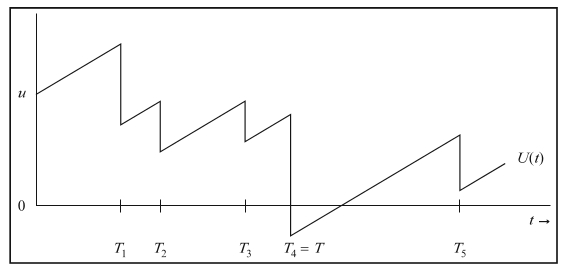
\includegraphics[scale=0.41]{Figuras/Ruin_Process.jpeg}
		\end{figure}
		{\tiny Fuente: Kaas et al.}
		\end{block}  		
	
\end{frame}

%
%	Sub-section: Antecedentes
%
\subsection{1.4. Teor\'ia de ruina: Un ejemplo}
%	-------------		FRAME		--------------------
\begin{frame}[fragile]
	\frametitle{1.4 Teoria de ruina: Un ejemplo}
	\scriptsize  	
		
		\vspace{0.1cm}
		\begin{block}<+->{Reaseguro (un escenario)}
		\vspace{0.1cm}
		Elaboramos sobre la conexi\'on entre \textcolor{blue}{\bf reaseguro} y \textcolor{blue}{\bf solvencia} (un ejemplo):
		\begin{itemize}
		  \item Una compa\~n\'ia se seguros deposita $U$ capital inicial y suscribe $J$ riesgos i.i.d. 
		  \item La prima de riesgo {\it individual} se fija seg\'un el \textcolor{blue}{principio del valor esperado}
		  \begin{equation}
		  \Pi_X = (1 + \rho) \expec_{F_X}(X).
		  \end{equation}
		  
		  \textcolor{red}{\bf Lo veremos en un momento...}
		  \item Definimos $S$ el monto agregado de p\'erdida. La \textcolor{blue}{probabilidad de ruina} de la compa\~n\'ia de seguros, se define como
		  \begin{eqnarray}
		  \psi 
		    & = &
		    \Pr\left( C + J (1+\rho)\expec_{F_X}(X)-S < 0\right)
		    \nonumber \\
		    & = &
		    \Pr\left( S - J\expec_{F_X}(X) > C+ J\rho\expec_{F_X}(X) \right).
		    \nonumber
		  \end{eqnarray}
		\end{itemize}
		\end{block}
		
\end{frame}


%	-------------		FRAME		--------------------
\begin{frame}[fragile]
	\frametitle{1.4 Teoria de ruina: Un ejemplo}
	\scriptsize  	
		
		\vspace{0.1cm}
		\begin{block}<+->{Reaseguro (un escenario)}
		\vspace{0.1cm}
		\begin{itemize}
		\item Por la desigualdad de Tchebychev,
		  \begin{equation}
		  \psi \leq 1/\beta^{2},
		  \nonumber
		  \end{equation}
		  donde
		  \begin{equation}
		  \beta = \frac{C+J\rho\expec(X)}{J^{1/2}d.e.(X)},
		  \nonumber
		  \end{equation}
		  es un coeficiente conocido como \textcolor{MyDarkGreen}{\bf coeficiente de seguridad} de la operaci\'on de la aseguradora.
		\end{itemize}
		\end{block}
		
\end{frame}

%	-------------		FRAME		--------------------
\begin{frame}[fragile]
	\frametitle{1.4 Teoria de ruina: Un ejemplo}
	\scriptsize  	
		
		\vspace{0.1cm}
		\begin{block}<+->{Reaseguro (un escenario)}
		\vspace{0.1cm}
		\begin{itemize}
		  \item La desigualdad anterior da una cota a la probabilidad de ruina, pero esta cota es demasiado {\bf conservadora}
		  \item Cuanto mayor sea $\beta$, menor ser\'a $\psi$ (probabilidad de ruina)
		  \item Para aumentar el coeficiente de seguridad, bajo una estructura de riesgo dada, es posible:
		  \begin{enumerate}
		  \scriptsize
		  \item[a)] Incrementar el capital $U$
		  \item[b)] Incrementar la suscripci\'on $J$
		  \item[c)] Incrementar la prima de riesgo {\it individual} a trav\'es de incrementar $\rho$
		  \end{enumerate}

		\end{itemize}
		\end{block}
		
\end{frame}

%	-------------		FRAME		--------------------
\begin{frame}[fragile]
	\frametitle{1.4 Teoria de ruina: Un ejemplo}
	\scriptsize  	
		
		\vspace{0.1cm}
		\begin{block}<+->{Reaseguro (un escenario)}
		\vspace{0.1cm}
		\begin{itemize}
		  \item[Obs.1] Para un $U$ dado, las opciones (b) y (c) son complicadas
		  \item[Obs.2] Para un $U$ dado, la \'unica manera de ajustar el coeficiente de seguridad en el corto plazo es actuar a trav\'es del reaseguro, i.e. \textcolor{blue}{alterar la estructura de riesgo} 
		  \item El \textcolor{blue}{\bf reaseguro} consiste en reducir $d.e.(X)$ (transferencia de riesgo) y disminuir $\rho$ (transferencia de utilidades) 
		  \begin{quote}
		  Determinar una estrategia \'optima de reaseguro consiste en arbitrar entre estos dos efectos, uno positivo y otro negativo.
		  \end{quote}
		\end{itemize}
		\end{block}
		
\end{frame}

%
%	Section: Modelo de Cr\'amer-L\"undberg
%
\section{2. Modelo de Cr\'amer-L\"undberg}
%	-------------		FRAME		--------------------
\begin{frame}[fragile]
\frametitle{}
\vspace{5.5cm}
\begin{flushright}
	\textcolor{MyDarkBlue}{\Large \bf 2. Modelo de Cr\'amer-L\"undberg}
\end{flushright}
\end{frame}

%
%	Sub-section: Antecedentes
%
\subsection{2.1. Modelo de Cr\'amer-L\"undberg: Fundamentos}
%	-------------		FRAME		--------------------
\begin{frame}[fragile]
\frametitle{2.1 Modelo de Cr\'amer-L\"undberg: Fundamentos}
\scriptsize  	

\vspace{0.1cm}
\begin{block}<+->{Antecedentes}
	\vspace{0.1cm}
	El modelo de Cr\'amer-L\"undberg (C-L) describe el valor neto de capital en el tiempo, $U_t$, de acuerdo a un {\bf proceso de riesgo},
	\begin{equation}
		U_t = U_0 + \Pi_t - S_t,
	\end{equation}
	donde
	\begin{itemize}
		\item[$U_0$] - capital inicial al tiempo $t=0$
		\item[$\Pi_t$] - suscripci\'on al tiempo $t0$
		\item[$S_t$] - reclamos totales al tiempo $t$.   
	\end{itemize}
\end{block}

\end{frame}


%	-------------		FRAME		--------------------
\begin{frame}[fragile]
\frametitle{2.1 Modelo de Cr\'amer-L\"undberg: Fundamentos}
\scriptsize  	

\vspace{0.1cm}
\begin{block}<+->{Supuestos}
	\vspace{0.1cm}
	Respecto a $S_t$, enfoque de {\bf riesgo colectivo}, i.e. 
	$$
	S_t=\sum_{j=1}^{N_t}X_j, 
	$$
	donde,
	\begin{itemize}
		\item[$N_t$] - proceso Poisson homog\'eneo con intensidad $\lambda > 0$
		
		\item[$X_j$s] - v.a.i.i.d. con $F_X(x)$ y $M_X(s)$ dadas tales que $\mathbb{E}(X_j)=\mu < \infty$.  
	\end{itemize}
	
	\vspace{0.1cm}
	Respecto a $\Pi_t$, enfoque de {\bf suscripci\'on continua}, $\Pi_t=\Pi t$
	\begin{itemize}
		\item[$\Pi$] - prima de riesgo instantanea, 
		$$
		\Pi=(1+\theta)\lambda\mu,
		$$
		con $\theta$ factor de recarga.
	\end{itemize}
\end{block}

\end{frame}

%
%	Sub-section: Antecedentes
%
\subsection{2.2. Modelo de Cr\'amer-L\"undberg: Definci\'on}

%	-------------		FRAME		--------------------
\begin{frame}[fragile]
\frametitle{2.2. Modelo de Cr\'amer-L\"undberg: Definci\'on}
\scriptsize  	

\vspace{0.1cm}
\begin{block}<+->{Definici\'on ruina}
	\vspace{0.1cm}
	Se define un episodio de {\bf ruina} cuando 
	$$
	U_t < 0.
	$$
	Asociado con esto, consideramos
	$$
	T=\inf\left\{t:U_t < 0\right\},
	$$
	como la variable de {\bf tiempo de ruina}.
\end{block}


\end{frame}


%	-------------		FRAME		--------------------
\begin{frame}[fragile]
\frametitle{2.2. Modelo de Cr\'amer-L\"undberg: Definci\'on}
\scriptsize  	

\vspace{0.1cm}
\begin{block}<+->{Probabilidades de inter\'es}
	\vspace{0.1cm}
	{\bf Probabilidad de ruina:}
	\begin{equation}
		\mathbb{P}(T < \infty) = \Psi(U_0).
	\end{equation}

	{\bf Probabilidad de ruina finita:}
	\begin{equation}
		\mathbb{P}(T < t) = \Psi(U_0,t).
	\end{equation}	
\end{block}

\begin{block}<+->{Objetivo}
	\vspace{0.1cm}
	\begin{quote}
		Calcular o acotar las probabilidades de ruina.
	\end{quote}
\end{block}

\end{frame}

%	-------------		FRAME		--------------------
\begin{frame}[fragile]
\frametitle{2.2. Modelo de Cr\'amer-L\"undberg: Coeficiente de L\"undberg}
\scriptsize  	

\vspace{0.1cm}
\begin{block}<+->{Definici\'on}
	\vspace{0.1cm}
	El {\bf coeficiente de L\"undberg} se define como la soluci\'on positiva de la ecuaci\'on
	\begin{equation}
		1+(1+\theta)\mu r = M_X(r)
	\end{equation}
	en t\'erminos de $r$. ({\it La soluci\'on no siempre existe}).
\end{block}

\vspace{0.1cm}
\begin{block}<+->{Equivalencias}
	\begin{eqnarray}
		\lambda + \Pi r 
		  & = & \lambda M_X(r),
		\nonumber
	\end{eqnarray}
	o,
	\begin{eqnarray}
	\Pi 
		& = &
		\frac{\log M_S(r)}{r},
		\nonumber
	\end{eqnarray}
	para 
	$$
	\Pi = (1+\theta)\lambda\mu.
	$$
\end{block}

\end{frame}

%
%	Sub-section: Antecedentes
%
\subsection{2.3. Modelo de Cr\'amer-L\"undberg: Cota}

%	-------------		FRAME		--------------------
\begin{frame}[fragile]
\frametitle{2.3. Modelo de Cr\'amer-L\"undberg: Cota}
\scriptsize  	

\vspace{0.1cm}
\begin{block}<+->{Definici\'on}
	\vspace{0.1cm}
	Si la soluci\'on para $r$ existe en las ecuaciones anteriores, se sigue que las {\bf probabilidades de ruina} pueden acotarse por
	\begin{equation}
	 \Psi(U_0,t) \leq \Psi(U_0) \leq \exp\{-r U_0\}.
	\end{equation}
	Se define as\'i a la cota de L\"undberg de la probabilidad de ruina.
\end{block}

\vspace{0.1cm}
\begin{block}<+->{Probabilidad de ruina}
	\vspace{0.1cm}
	Adicionalmente, la probabilidad de ruina puede definirse como
	\begin{eqnarray}
	\Psi(U_0) 
	  & = & \frac{\exp\{-r U_0\}}{\mathbb{E}_{F_{S_t}}\left(\exp\{-r C_T\} | T<\infty\right)}
	  \leq 
	  \exp\{-r U_0\}.
	\nonumber
	\end{eqnarray}
 	El denominador $\mathbb{E}_{F_{S_t}}(\exp\{-r C_T\}| T<\infty)$ es mayor a 1, cuando $r$ existe.
\end{block}


\end{frame}

%
%	Sub-section: Antecedentes
%
\subsection{2.4. Modelo de Cr\'amer-L\"undberg: Inexistencia}

%	-------------		FRAME		--------------------
\begin{frame}[fragile]
\frametitle{2.4. Modelo de Cr\'amer-L\"undberg: Inexistencia}
\scriptsize  	

\vspace{0.1cm}
\begin{block}<+->{Condici\'on}
	\vspace{0.1cm}
	En el modelo C-L, la ecuaci\'on que define la existencia de la cota de L\"undberg tiene soluci\'on no negativa si y s\'olo si 
	\begin{equation}
	\int_{0}^{\infty}\exp\{rx\} F_X(dx)<\infty 
	\label{eq_tail}
	\end{equation}
	al rededor de $0$ en t\'erminos de $r$.

	\begin{itemize}
	  \item Esta condici\'on se satisface si,
		$$
		\frac{1-F_X(x)}{\exp\{-r x\}} \leq \mathbb{E}_{F_X}(\exp\{rX\}).
		$$

	  \item \textcolor{MyDarkGreen}{La cola de la distribuci\'on $F_X$ debe estar acotada exponencialmente.}
	\end{itemize}
\end{block}

\end{frame}

%
%	Sub-section: Antecedentes
%
\subsection{2.5. Modelo de Cr\'amer-L\"undberg: Comentarios}

%	-------------		FRAME		--------------------
\begin{frame}[fragile]
\frametitle{2.5. Modelo de Cr\'amer-L\"undberg: Comentarios}
\scriptsize  	

\vspace{0.1cm}
\begin{block}<+->{Comentarios}
	\vspace{0.1cm}
	El modelo de C-L es un modelo que descansa en supuestos estrictos de
	\begin{itemize}
	  \item {\bf homogeneidad temporal}
	  \item {\bf homogeneidad de riesgos (dentro del portafolio)}
	  \item {\bf previsi\'on moderada de riesgos individuales}.
	\end{itemize}
	Estos supuestos hacen que los c\'aculos anal\'iticos sean posibles de obtener.
\end{block}

\vspace{0.1cm}
\begin{block}<+->{Consideraciones pr\'acticas}
	\vspace{0.1cm}
	En la {\bf pr\'actica}, muchos de estos supuestos tienen que relajarse; en cuyo caso, c\'aculos basados en aproximaciones asint\'oticas, anal\'iticas y/o num\'ericas ser\'an requeridos.
\end{block}


\end{frame}

\end{document}
%
%	--	FIN	--